\documentclass[12pt,a4paper, titlepage]{article}
\usepackage{amsmath}
\usepackage{graphicx}
\usepackage{float}
\usepackage{wrapfig}
\usepackage[russian]{babel}
\usepackage[utf8]{inputenc}


\title{Работа 1. Анализ результатов численного моделирования обтекания пластины, скругленной по цилиндру}
\date{2021\\Сентябрь}
\author{Петраков Иван\\\ МФТИ\\\\\\\\\\\\\\\\\\\\}
\hoffset = 0pt
\voffset = 0pt
\textheight = 700pt
\topmargin = 0pt
\headheight = 0pt
\headsep = 0pt
\marginparwidth = 0pt
\oddsidemargin = 0pt
\textwidth = 450pt

\begin{document}

\maketitle

\subsection*{Описание задачи}
\noindent\rule{\textwidth}{1pt}
Имеется пластина, скругленная у кромки. Она обтекается совершенным газом, направленным параллельно пластине. Заданы параметры газа: число Маха $M = 1.5$ и число Рейнольдса $Re = 6 \cdot 10^6$.
\\
\\
В задаче требуется:
\\
1) построить и сравнить графики трения на пластине на сетках с разным первым пристеночным шагом и объяснить их расхождение;
\\
2) Сравнить профили скорости при решении задачи в рамках уравнения Эйлера и Навье-Стокса по нормали от т. (0,1) до (0, 1.01) и от т. (0, 1) до (0, 1.002) и объяснить расхождение;
\\
3) Исследовать график сходимости в зависимости от CFL для решения в рамках уравнения Навье-Стокса на сетке с шагом $10^{-6}$. Найти пограничное значение CFL, при увеличении которого не наблюдается ускорения сходимости.
\\
\\
Численные расчеты предлагалось делать с использованием уже скомпилированной программы. Изменение параметров для решения задач происходило в соответствующих .ini файлах. Расчет происходил на кластере в силу медленной работы последовательной версии программы.
\subsection*{Результаты работы}
\noindent\rule{\textwidth}{1pt}
Все результаты работы основаны на проведенных мной расчетах на кластере. Расчеты хранятся в папке Petrakov.
\\
\paragraph{Сравнение сил трения}
Построим график зависимости силы трения от координаты для разных первых пристеночных шагов. В нашем случае использовались следующие шаги: $10^{-3}$ и $10^{-6}$. Получим следующие результаты:
\begin{figure}[H]
	\centering
	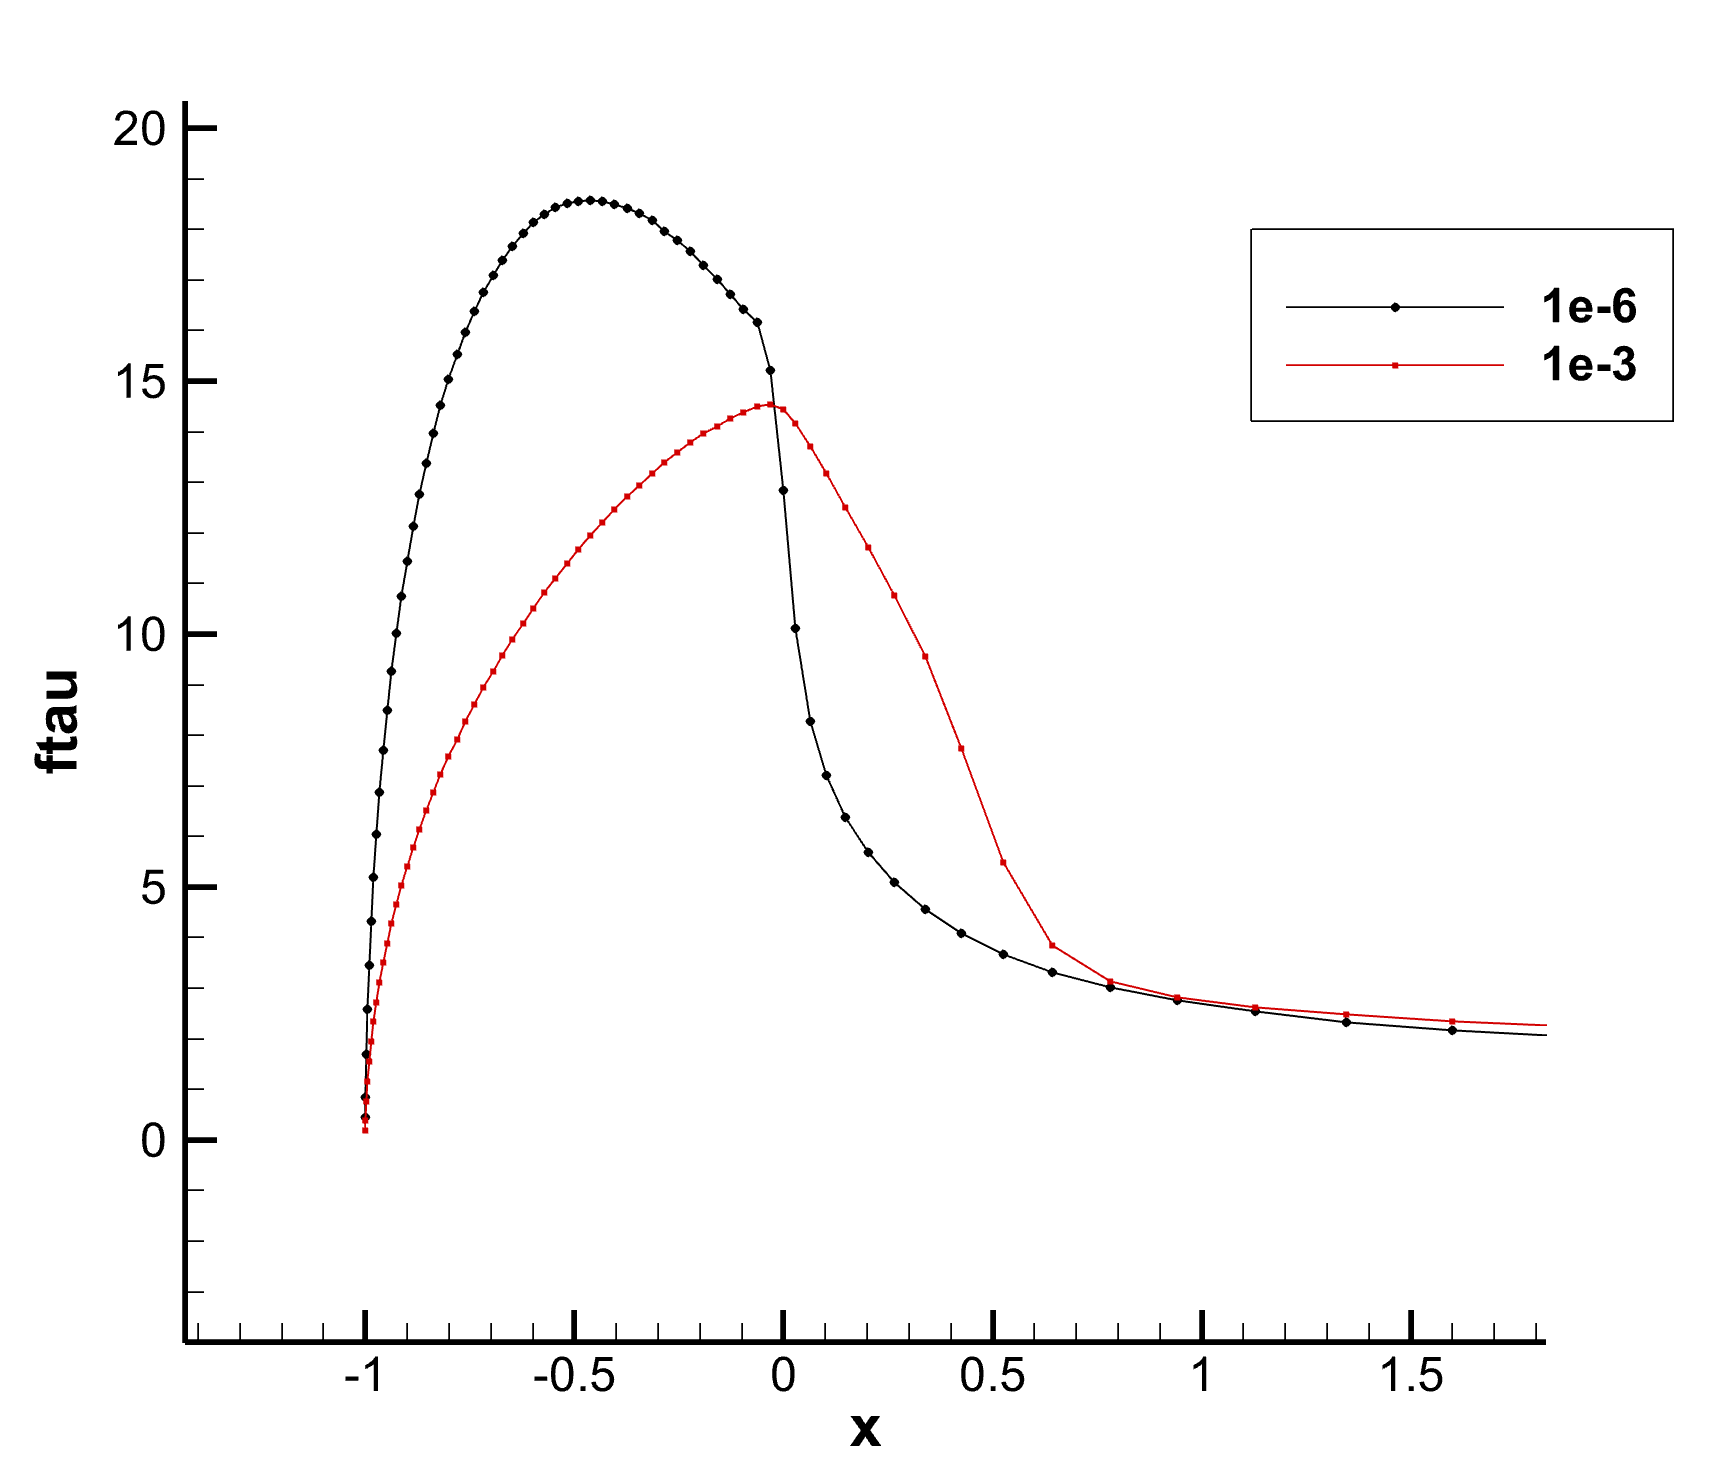
\includegraphics[width = 1.0\textwidth]{ans_1.png}
\end{figure}

\paragraph{Сравнение профилей скоростей}
Построим график зависимости скорости потока в направлении координаты $x$ от координаты $y$. Строить зависимости будем при/без учете/а вязкости, а также при разных пристеночных шагах. Получим следующие результаты:
\begin{figure}[H]
	\centering
	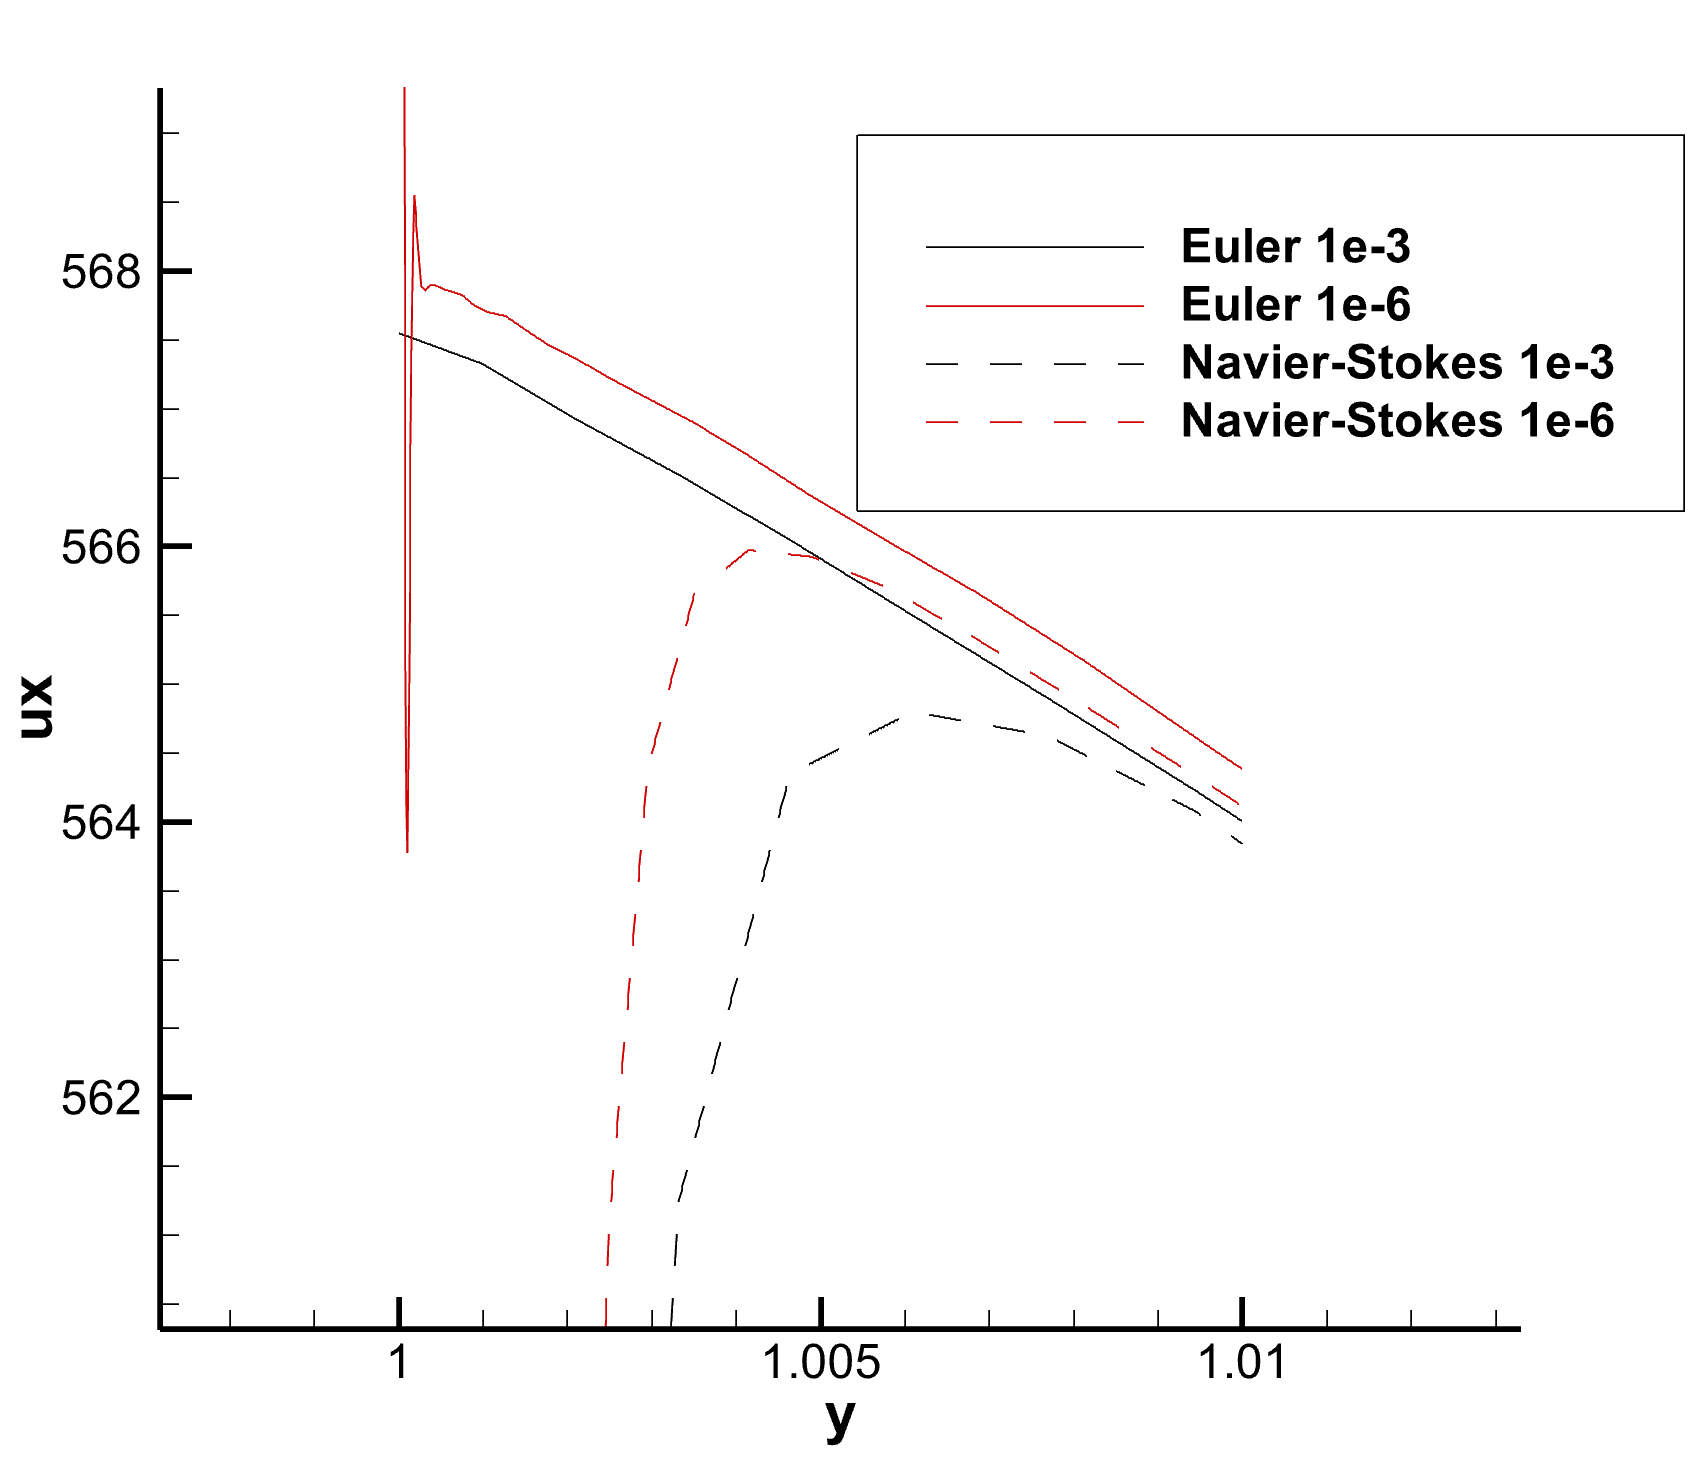
\includegraphics[width = 1.0\textwidth]{ans_2.png}
\end{figure}

Рассмотрим также графики зависимости скорости потока в напавлении координаты $x$ от координаты $y$ в рамках уравнений Навье-Стокса и Эйлера для одного значения первого пристеночного шага ($10^{-6}$). Получим следующие результаты:
\begin{figure}[H]
	\centering
	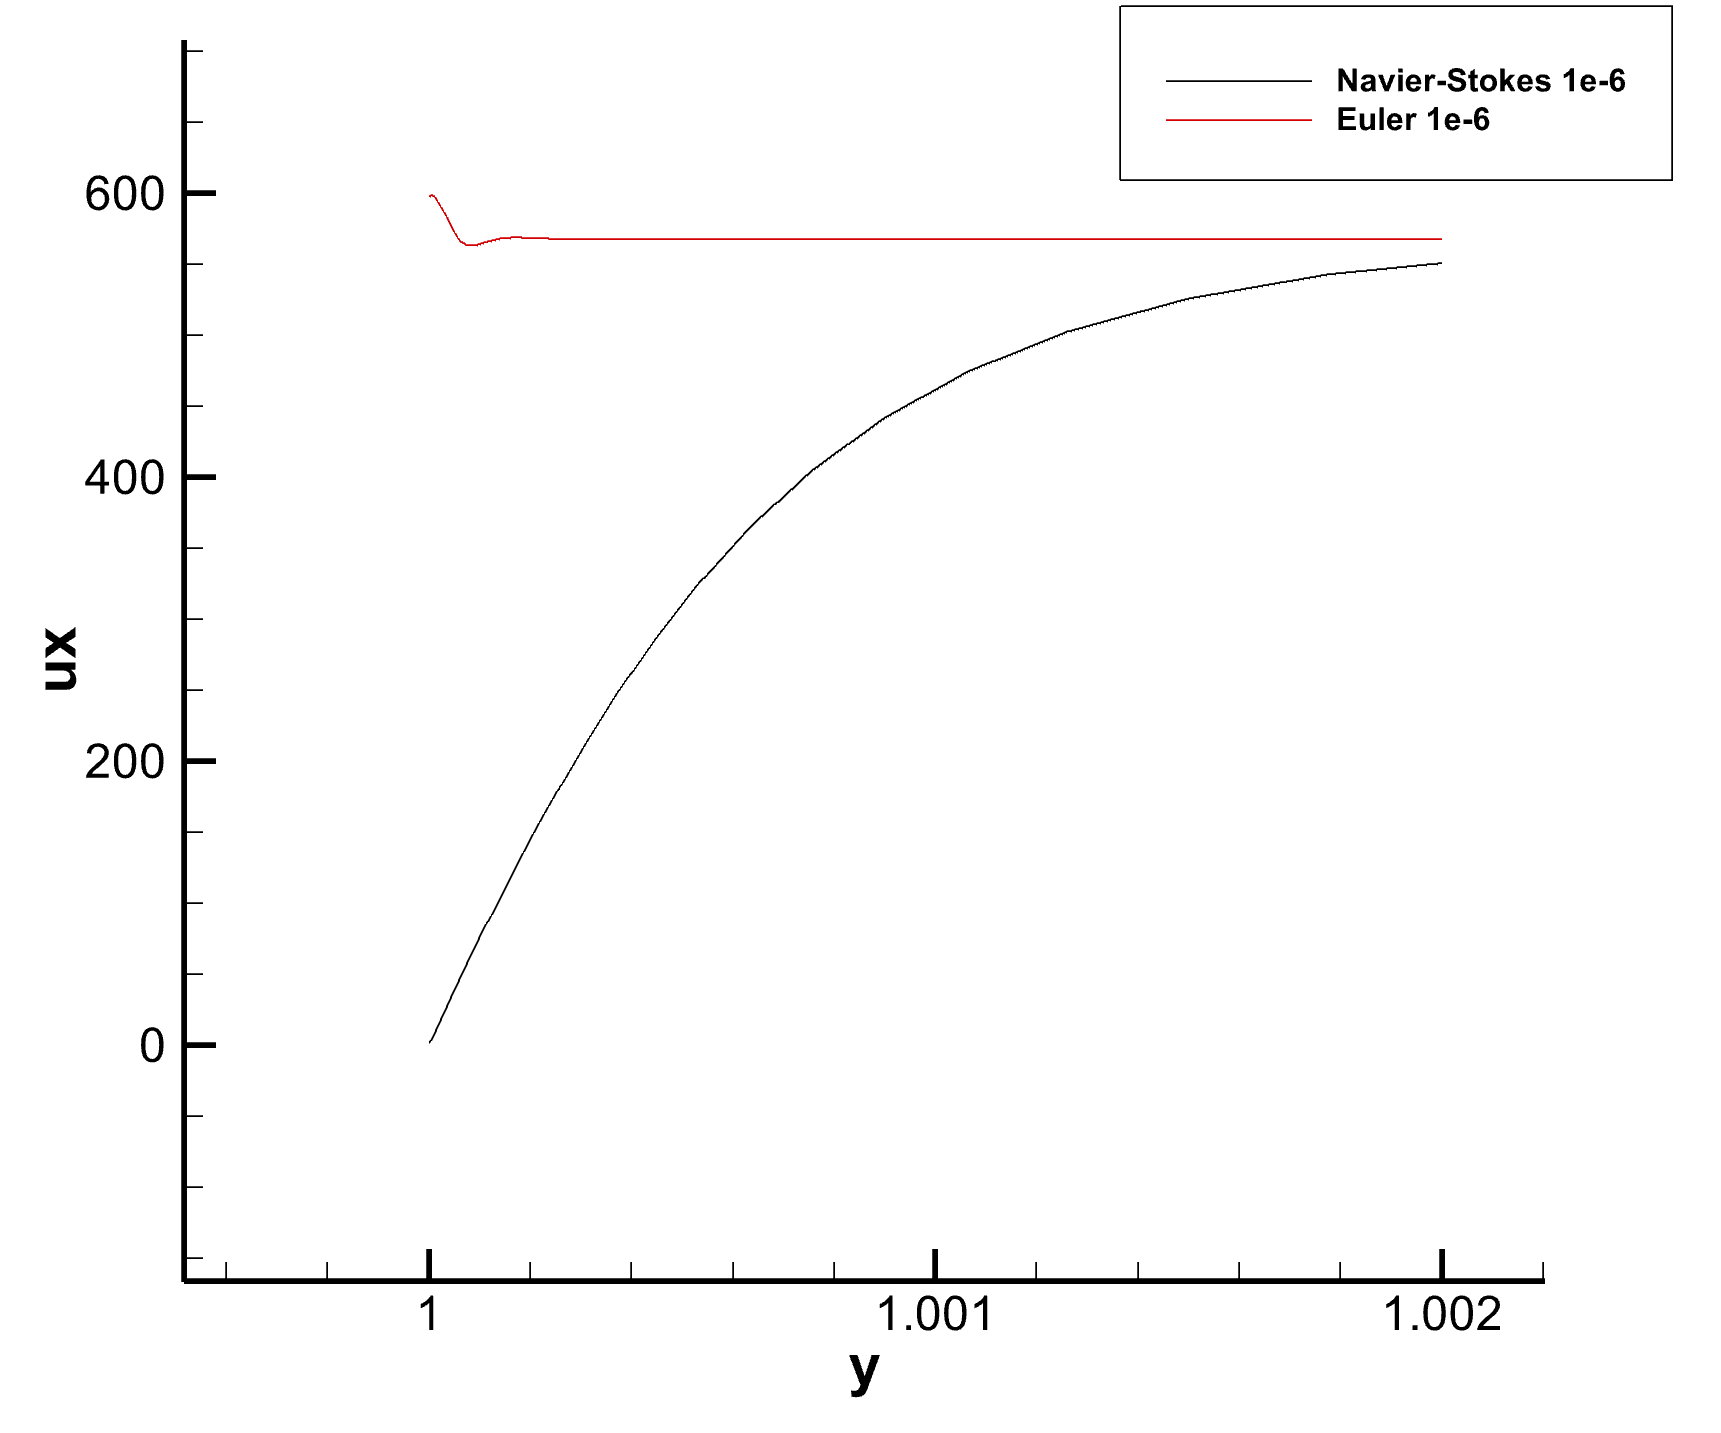
\includegraphics[width = 1.0\textwidth]{ans_2_add.png}
\end{figure}

\paragraph{Исследование на критическое значение CFL}
Проведем расчеты в рамках уравнений Навье-Стокса и с первым пристеночным шагом, равным $10^{-6}$, в большом диапазоне CFL. Получим следующие результаты:
\begin{figure}[H]
	\centering
	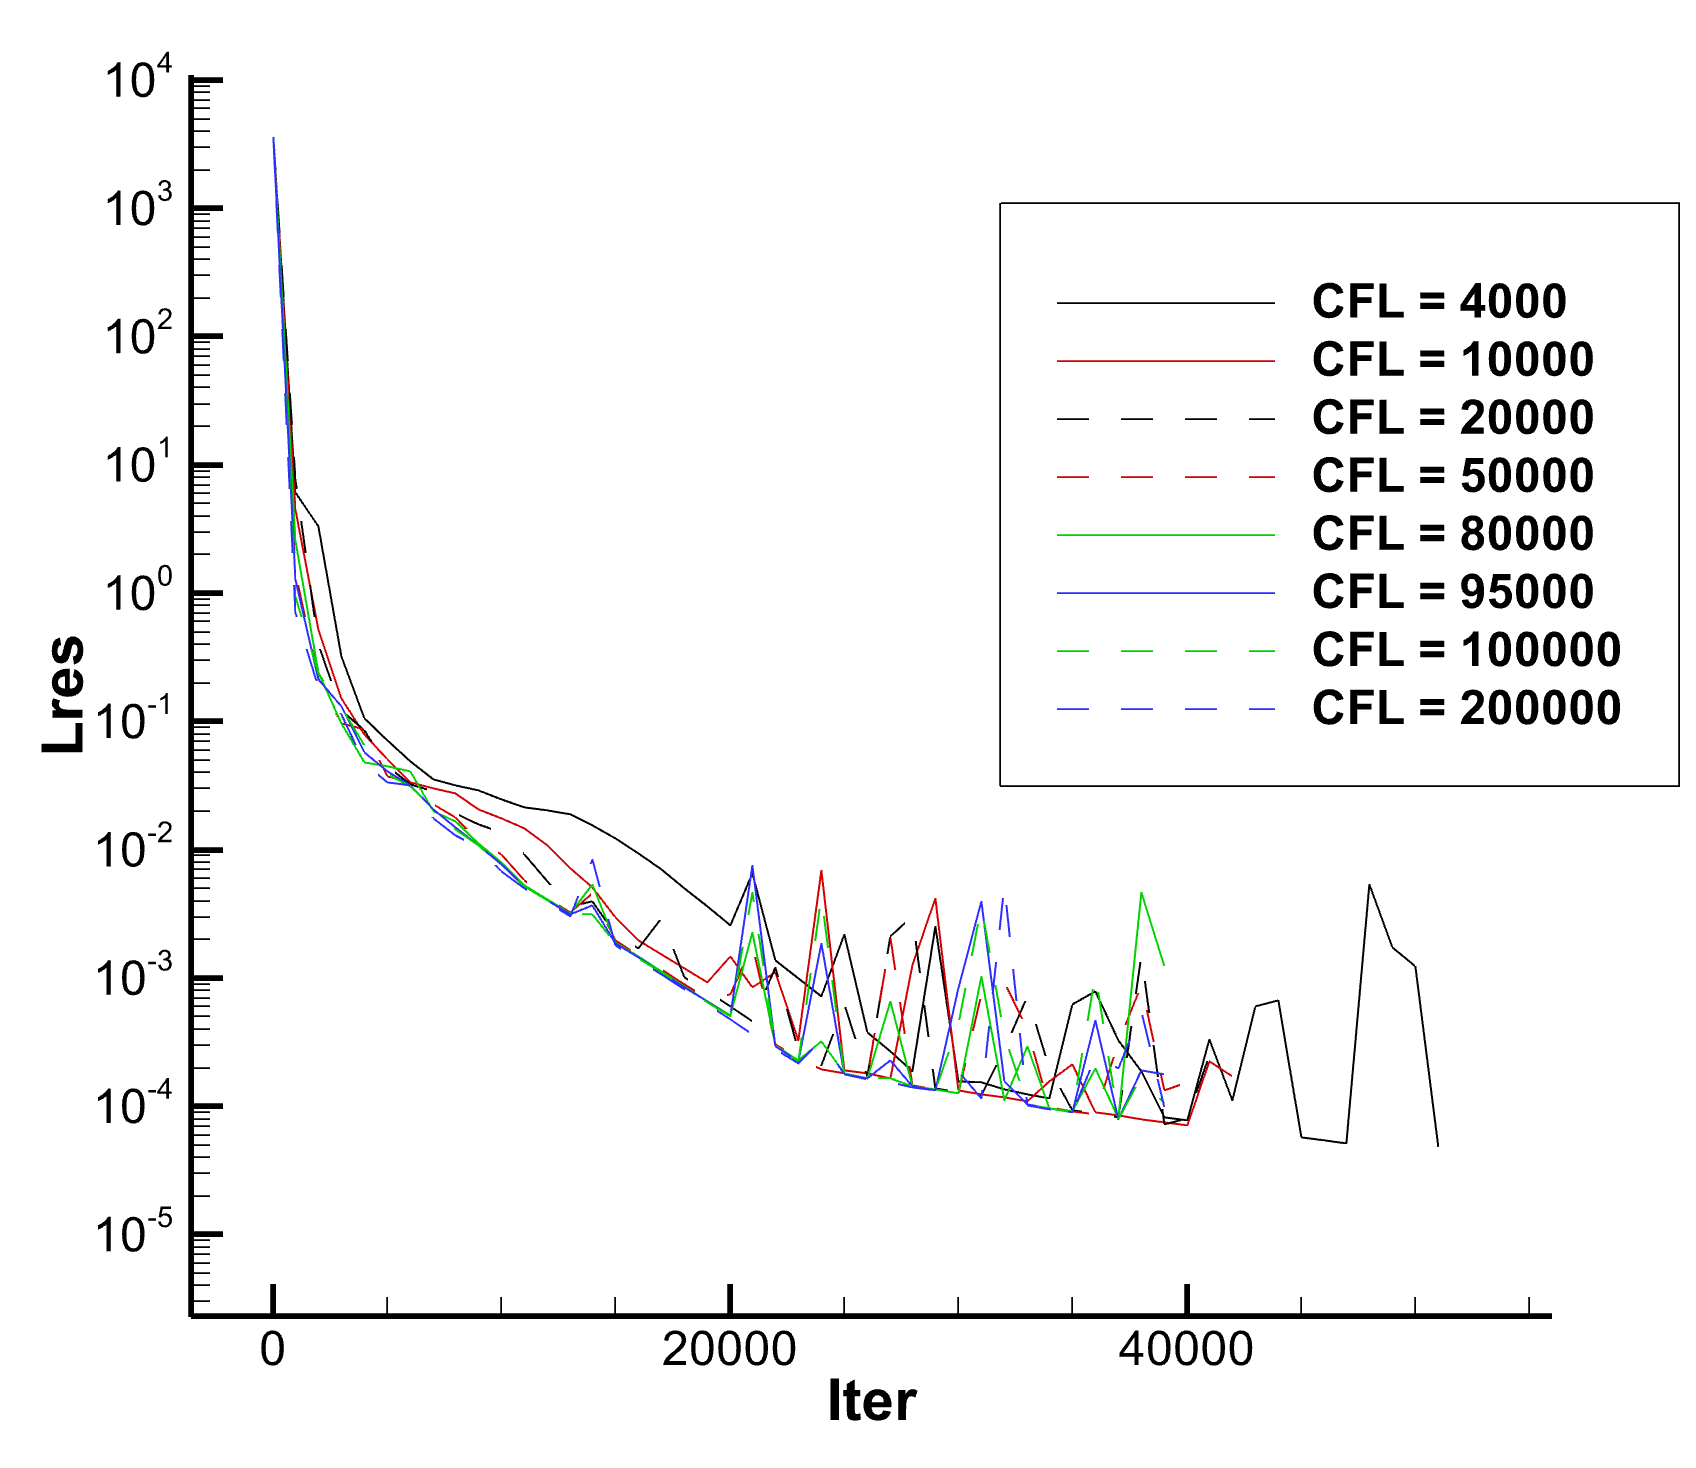
\includegraphics[width = 1.0\textwidth]{ans_3_full.png}
\end{figure}
Как видно, работать с такими данными очень сложно, поэтому выделим более-менее линейный участок, на котором и будем исследовать ускорение сходимости, а также участок графика, где достигается необходимая погрешность (для определения количества итераций). Получим следующие результаты:
\begin{figure}[H]
	\centering
	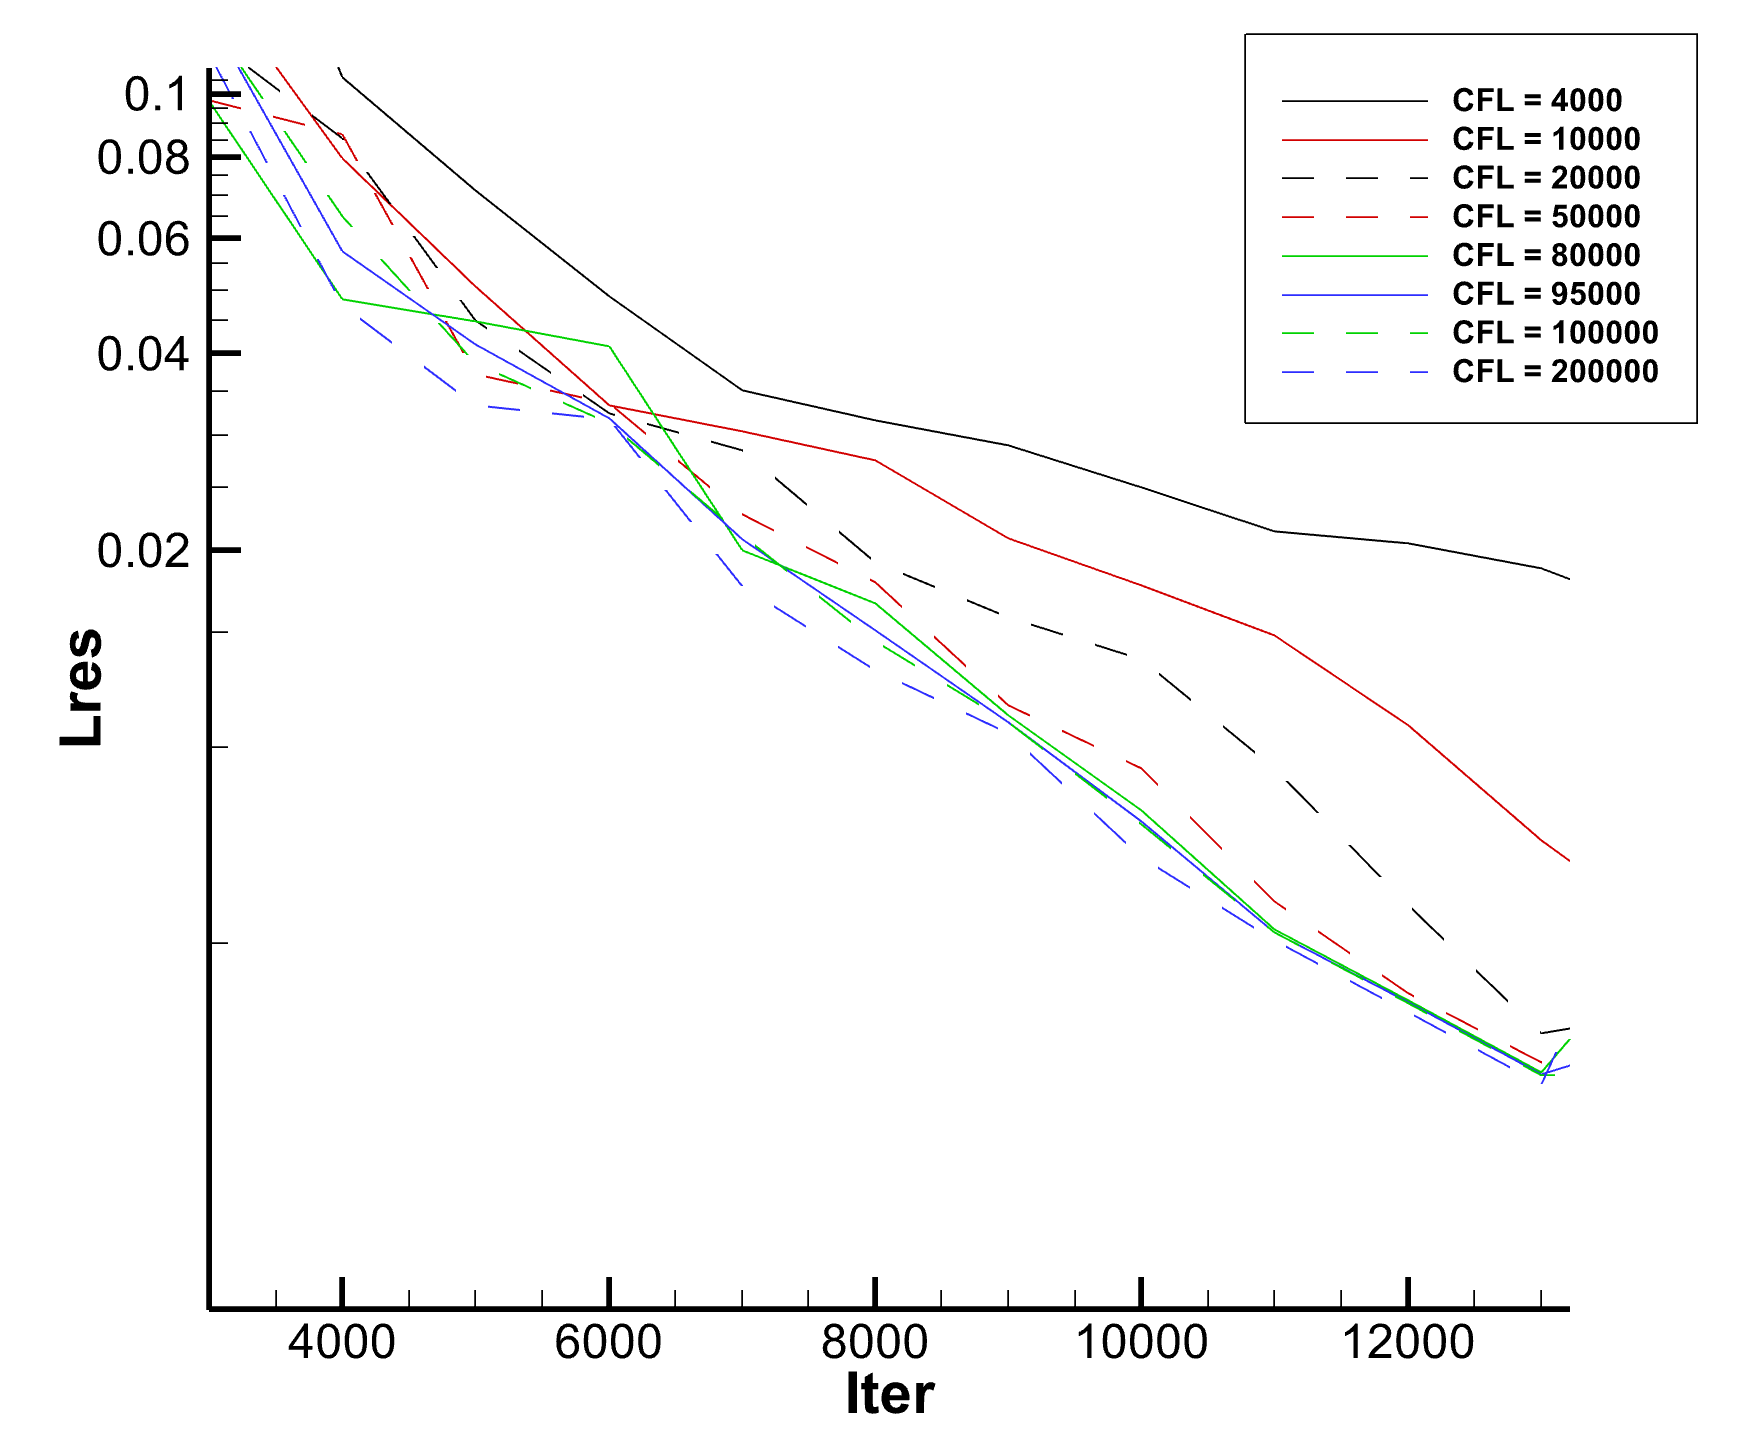
\includegraphics[width = 1.0\textwidth]{ans_3_short.png}
\end{figure}
\begin{figure}[H]
	\centering
	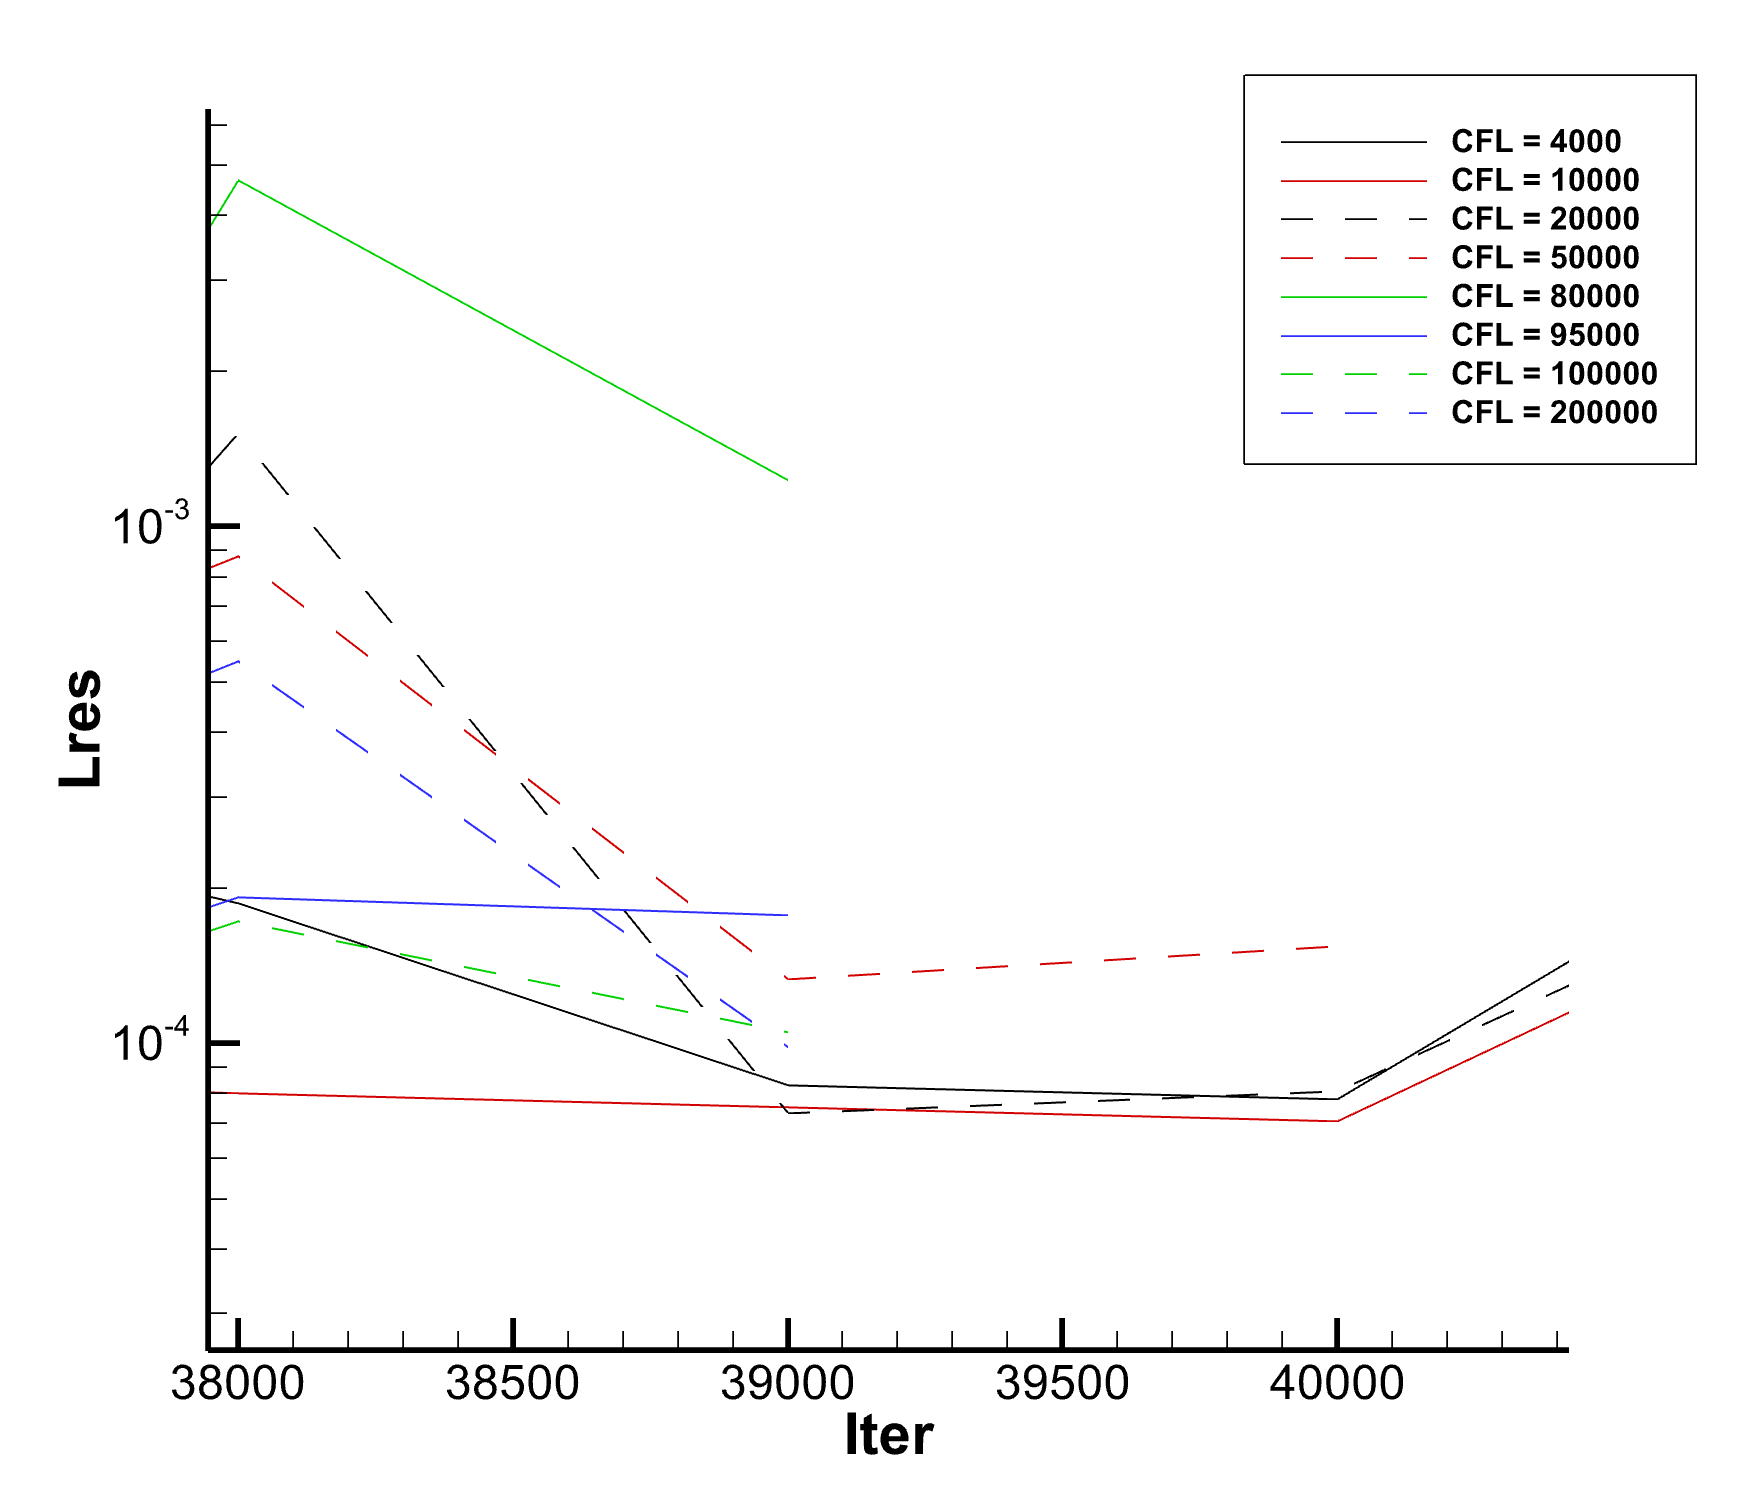
\includegraphics[width = 1.0\textwidth]{ans_3_end.png}
\end{figure}

\subsection*{Обсуждения результатов}
\noindent\rule{\textwidth}{1pt}
\paragraph{Сравнение сил трения}
Не сложно заметить расхождение в двух графиках. Видно, что они выходят на какую-то постоянную одинаковую величину, однако максимально достигаемое значение силы трения отличается. Обратимся к степенному закону вязкости жидкости. Для неньютоновской жидкости он выглядит как
\begin{equation}
	\tau = K (\frac{\partial u}{\partial y})^n
\end{equation}
где $K$ - коэффициент густоты потока, $n$ - показатель поведения жидкости, $u$ - скорость потока, параллельного стенке, $y$ - расстояние до стенки.
\\
В общем случае, имеем немного другое уравнение
\begin{equation}
	\tau = \mu (\frac{\partial u}{\partial y})|_{y = 0}
\end{equation}
где $\mu$ - динамическая вязкость.
\\
Считая первый пристеночный шаг достаточно малым (что и присутствует в наших расчетах), скорость прямо у стенки нулевой, получим, что частные производные можно заменить приращением. Тогда, в итоге, сила трения обратно пропорциональна расстоянию до стенки, что и отражено на графике. Достижение максимума в различных точках, возможно, связана с различной скоростью потока, а также с ошибкой, появившейся, когда мы заменяли частные производные.
\paragraph{Сравнение профилей скоростей}
Рассмотрим полученные зависимости скорости от координаты $y$. Из первого графика видно, что, действительно, скорость отличается в зависимости от значения первого пристеночного шага, что подтверждает выводы, сделанные в предыдущем параграфе. Из первого и второго графика видно, что зависимости ведут себя по-разному, в зависимости от того, в условиях каких уравнений мы решаем задачу. Расхождение связано с наличием вязкости (а следовательно, вязкого трения) при решении задачи в условиях уравнений Навье-Стокса, что и отражается на графиках (резкое снижение скорости). В случае уравнения Эйлера, скорость достигается сразу максимальная. Оба графика показывают снижение скорости в зависимости от расстояния от пластинки, что подтверждается курсом механики сплошных сред.
\paragraph{Исследование на критическое значение CFL}
Как было сказано в предыдущем разделе, обсуждать первый график нет никакого смысла - он не особо информативный. Рассмотрим второй график. Очевидно, что чем ниже кривая, тем быстрее сходимость. Наблюдаем увеличение скорости сходимости при увеличении CFL. Однако, есть некоторые точки (Iter = 6000, 9000, 13000), в которых значения Lres для последних трех чисел CFL совпадает. Это может косвенно говорить нам о достижении критического значения CFL, после которого не наблюдается увеличения скорости сходимости (дело в том, что если провести через совпадающие точки прямые, то получим одинаковый наклон у каждого графика, что и говорит об одинаковой скорости сходимости). 
\\
Теперь рассмотрим последний в работе график. Видно, что для последних 4х чисел CFL график обрывается на одном и том же значении, что говорит о достижении поставленной погрешности.
\\
Исходя из данных выводов, можно сделать предположение о критическом CFL, равным около 100000. Считаю, что находить ошибку определения данного значения в рамках данной задаче не имеет смысла - это требовало бы более длительных расчетов на большем количестве чисел CFL.
\subsection*{Выводы}
\noindent\rule{\textwidth}{1pt}
В работе были решены поставленные задачи с использованием предоставленной программе, объяснены расхождения между некоторыми результатами, а также было найдено критическое значение CFL, при увеличении которого не наблюдается ускорения сходимости.


\end{document}